\documentclass{article}
\usepackage{amsmath,graphicx}
\begin{document}
\title{Time evolution of mode-summed radial self-force of a scalar field on an eliptical orbit in a Schwarszchild background using extrapolations in both the mode-sum and the Discontinuous Galerkin error}
\author{Steven Dorsher, Peter Diener, Frank L\"{o}ffler}
\maketitle


\section{New stuff}

From yesterday, Peter has asked me to
\begin{enumerate}
\item Re-examine each $F_{\inf}$ for each mode and be sure that it is not discontinuous using the median
\item Do the sum for individual values of lmin and lmax
\item Repeat this for many lmin and lmax and take the average and the standard deviation to get the spread
\end{enumerate}

\subsection{1. Checking for discontinuities in $F_{\inf}$ for each each l-mode}

There are no discontinuities in $F_{\inf}$ for any of the l-modes. See attached figures zero through thirty.

\begin{figure}
  \includegraphics{/home/sdorsher/LabNotebook/20170727/finfovertimel0}
\end{figure}

\begin{figure}
  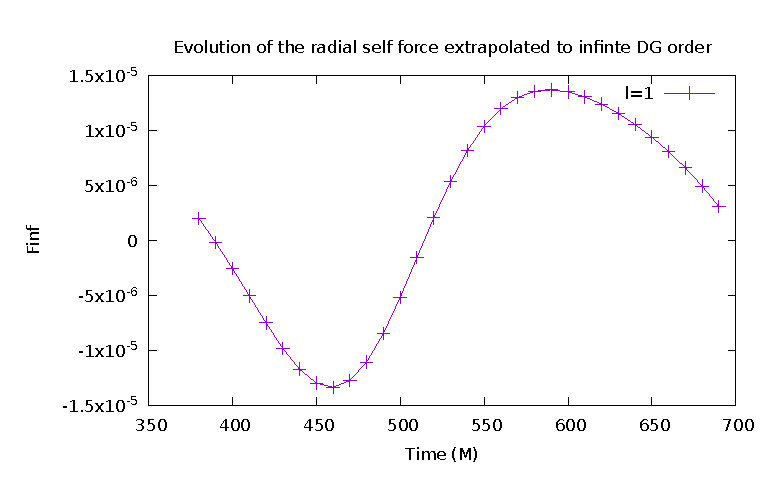
\includegraphics{/home/sdorsher/LabNotebook/20170727/finfovertimel1}
\end{figure}

\begin{figure}
  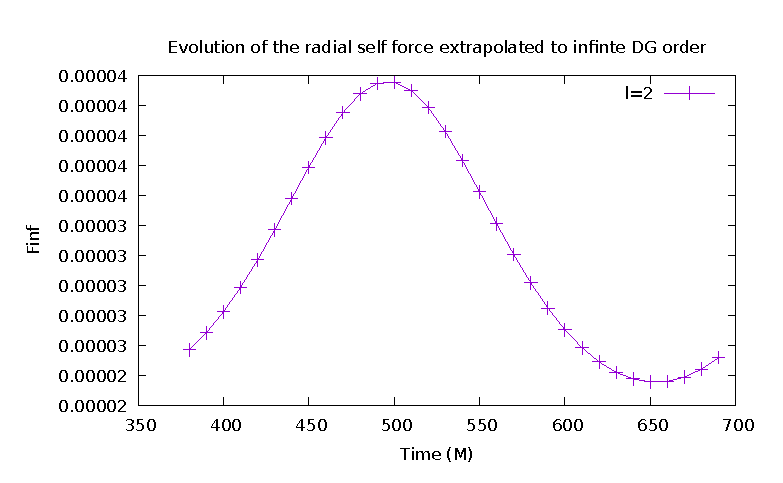
\includegraphics{/home/sdorsher/LabNotebook/20170727/finfovertimel2}
\end{figure}

\begin{figure}
  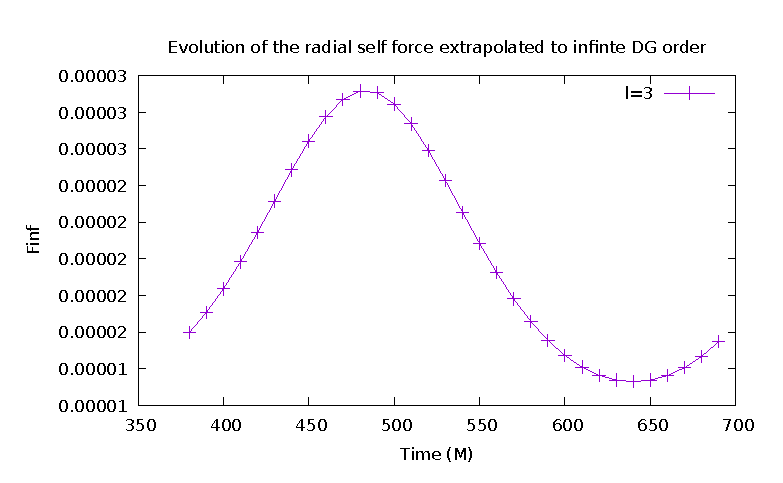
\includegraphics{/home/sdorsher/LabNotebook/20170727/finfovertimel3}
\end{figure}

\begin{figure}
  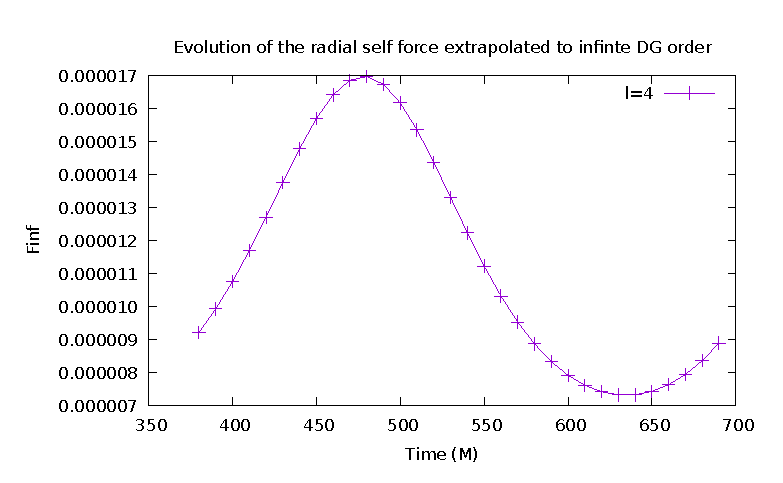
\includegraphics{/home/sdorsher/LabNotebook/20170727/finfovertimel4}
\end{figure}

\begin{figure}
  \includegraphics{/home/sdorsher/LabNotebook/20170727/finfovertimel5}
\end{figure}

\begin{figure}
  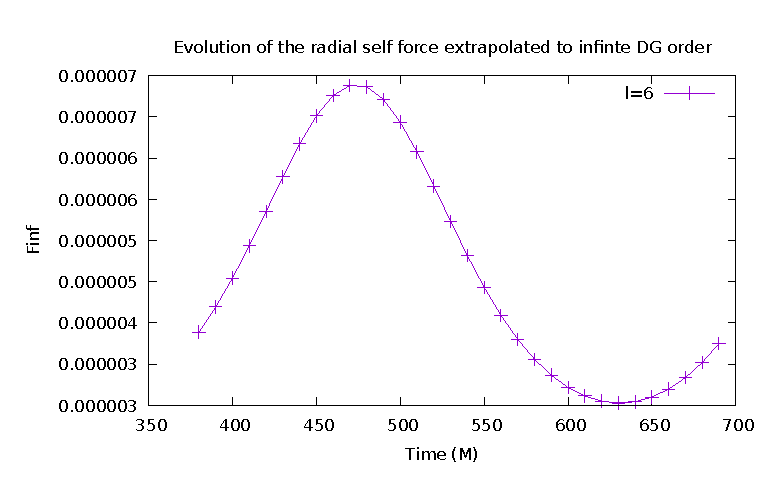
\includegraphics{/home/sdorsher/LabNotebook/20170727/finfovertimel6}
\end{figure}

\begin{figure}
  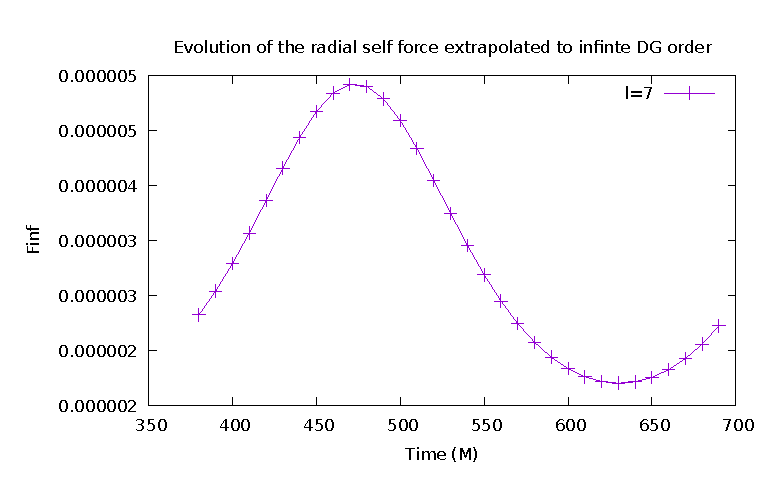
\includegraphics{/home/sdorsher/LabNotebook/20170727/finfovertimel7}
\end{figure}




\begin{figure}
  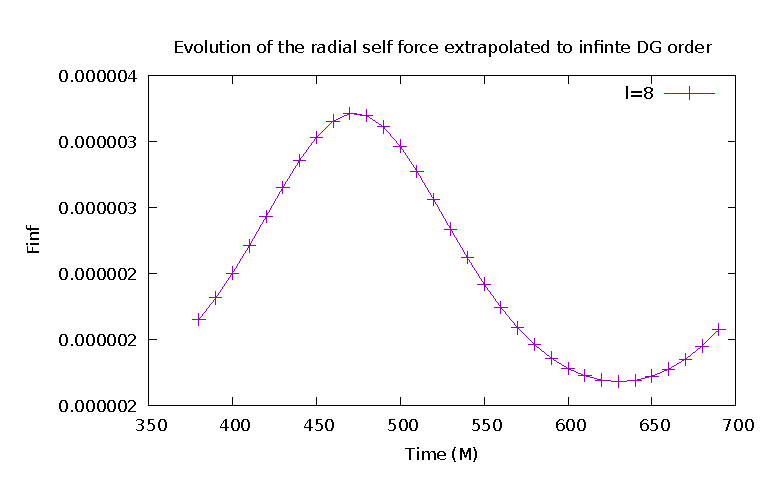
\includegraphics{/home/sdorsher/LabNotebook/20170727/finfovertimel8}
\end{figure}

\begin{figure}
  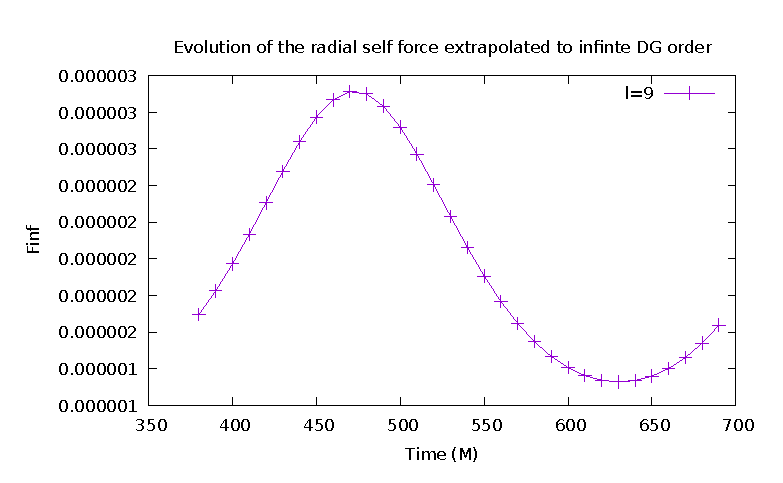
\includegraphics{/home/sdorsher/LabNotebook/20170727/finfovertimel9}
\end{figure}

\begin{figure}
  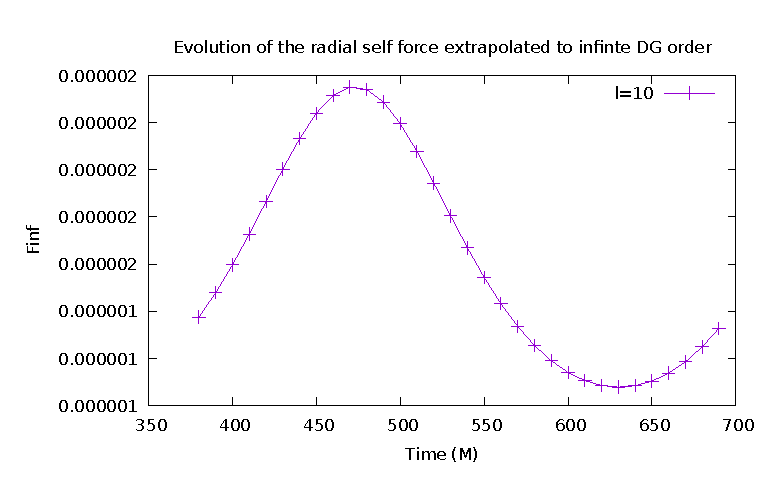
\includegraphics{/home/sdorsher/LabNotebook/20170727/finfovertimel10}
\end{figure}

\begin{figure}
  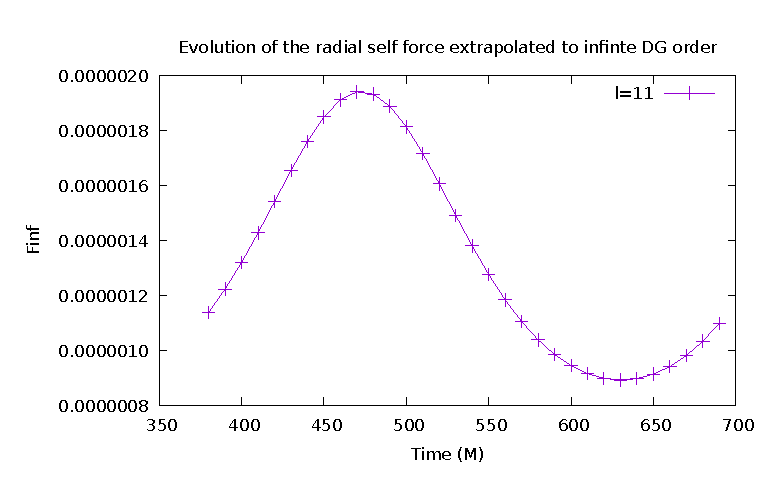
\includegraphics{/home/sdorsher/LabNotebook/20170727/finfovertimel11}
\end{figure}

\begin{figure}
  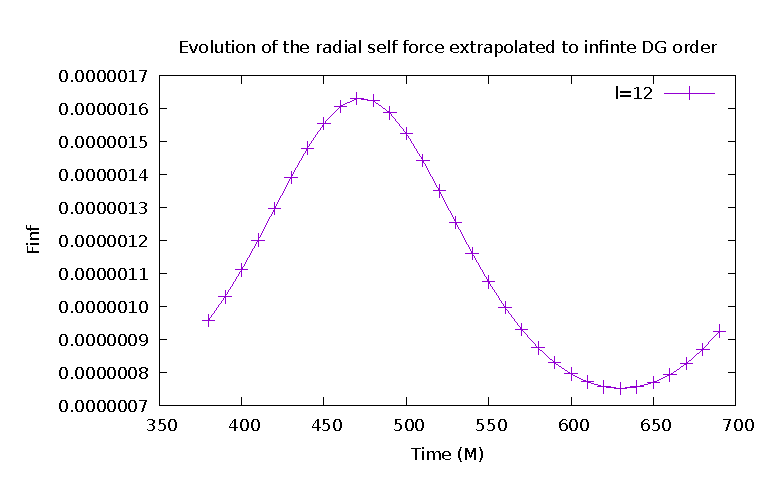
\includegraphics{/home/sdorsher/LabNotebook/20170727/finfovertimel12}
\end{figure}

\begin{figure}
  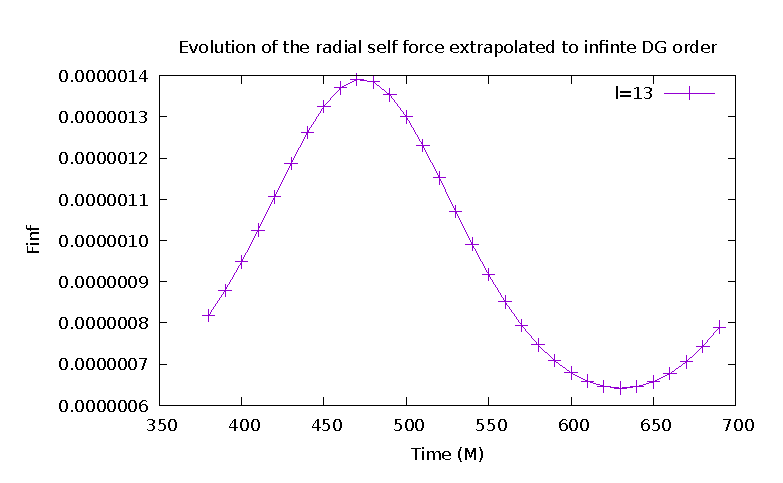
\includegraphics{/home/sdorsher/LabNotebook/20170727/finfovertimel13}
\end{figure}

\begin{figure}
  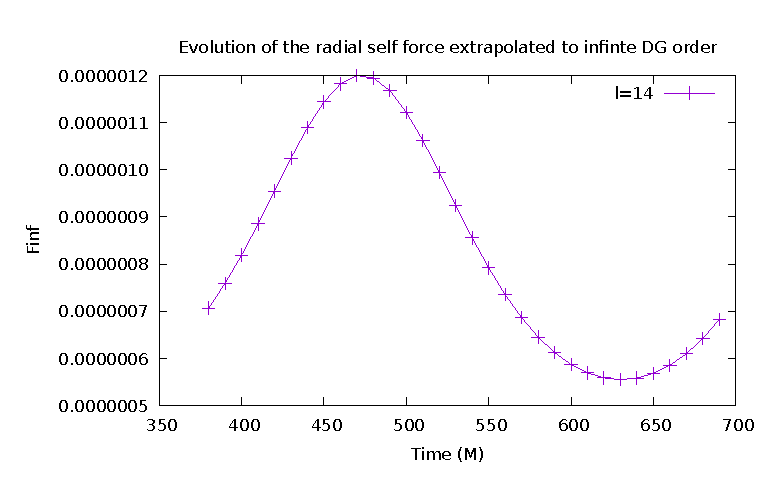
\includegraphics{/home/sdorsher/LabNotebook/20170727/finfovertimel14}
\end{figure}

\begin{figure}
  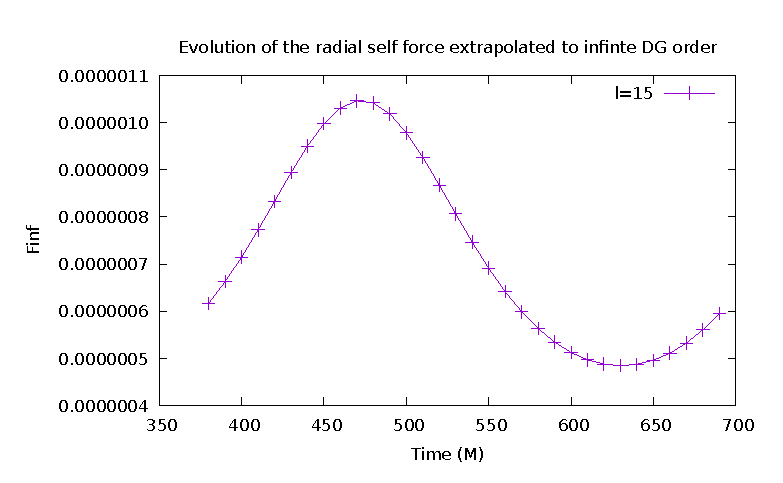
\includegraphics{/home/sdorsher/LabNotebook/20170727/finfovertimel15}
\end{figure}

\begin{figure}
  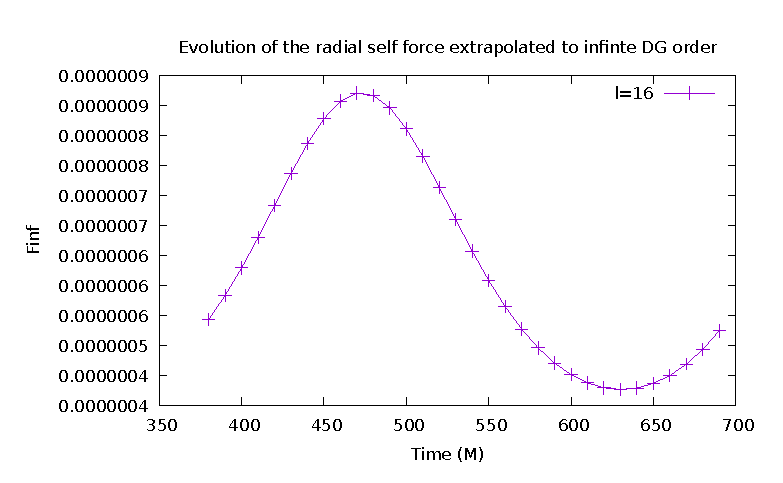
\includegraphics{/home/sdorsher/LabNotebook/20170727/finfovertimel16}
\end{figure}

\begin{figure}
  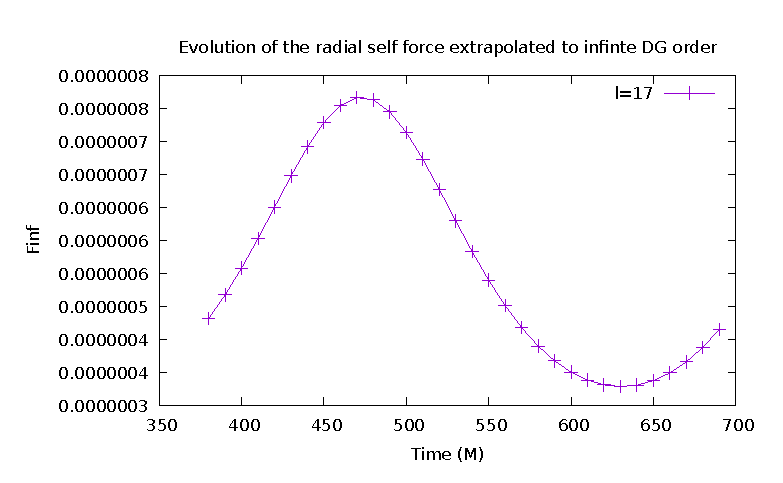
\includegraphics{/home/sdorsher/LabNotebook/20170727/finfovertimel17}
\end{figure}

\begin{figure}
  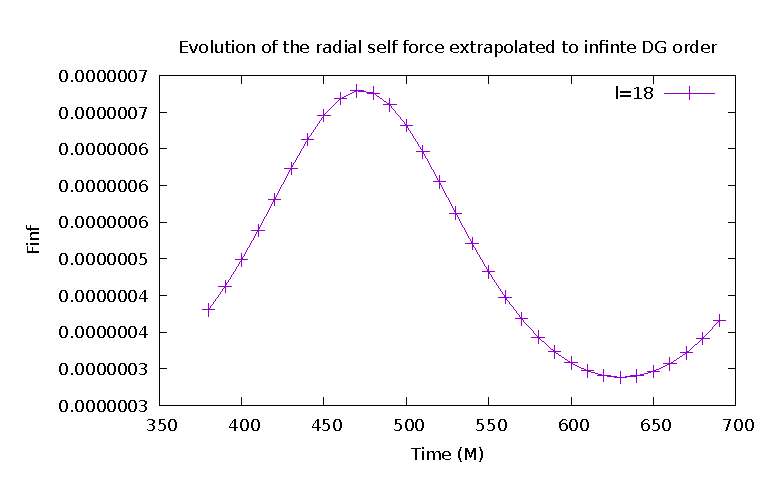
\includegraphics{/home/sdorsher/LabNotebook/20170727/finfovertimel18}
\end{figure}

\begin{figure}
  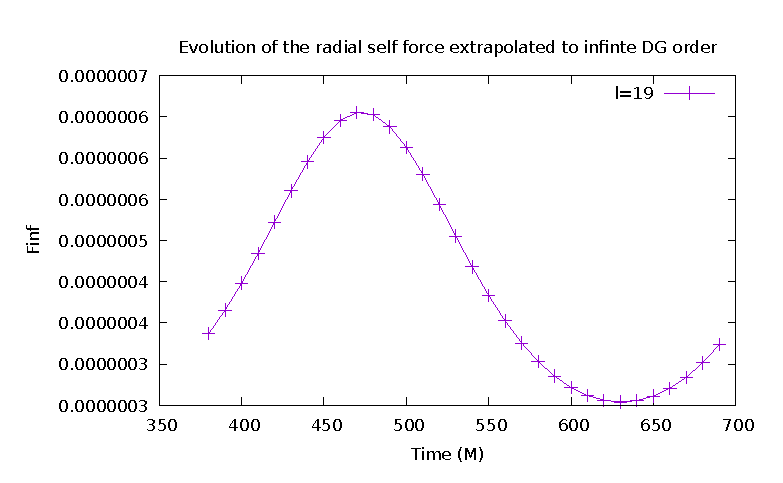
\includegraphics{/home/sdorsher/LabNotebook/20170727/finfovertimel19}
\end{figure}

\begin{figure}
  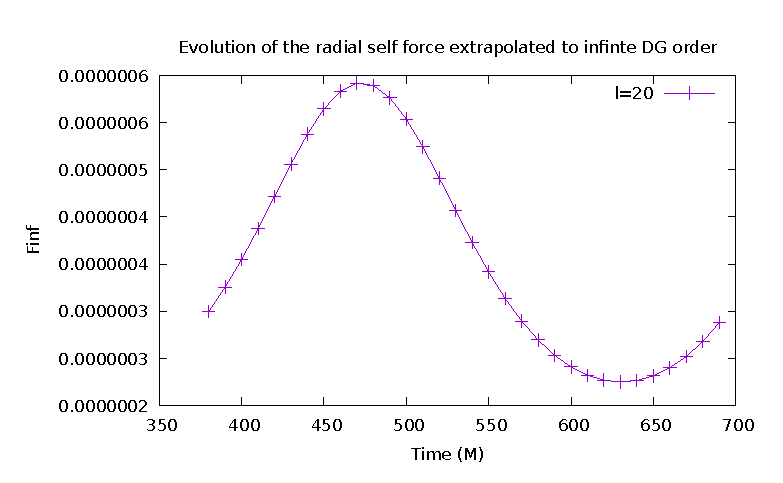
\includegraphics{/home/sdorsher/LabNotebook/20170727/finfovertimel20}
\end{figure}

\begin{figure}
  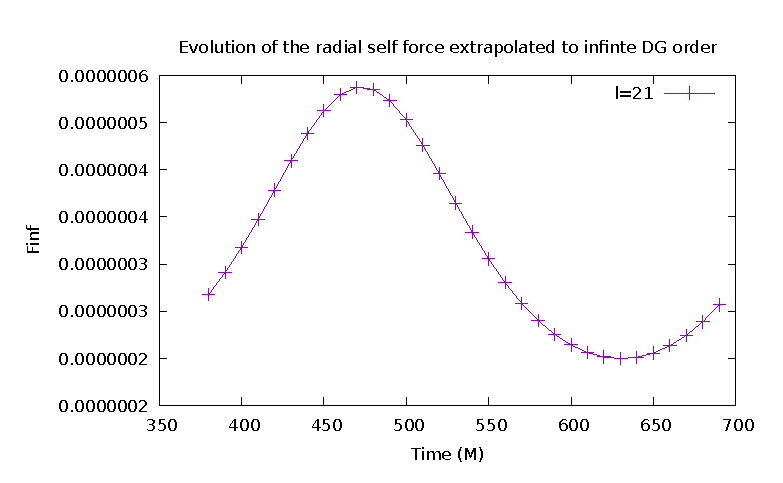
\includegraphics{/home/sdorsher/LabNotebook/20170727/finfovertimel21}
\end{figure}

\begin{figure}
  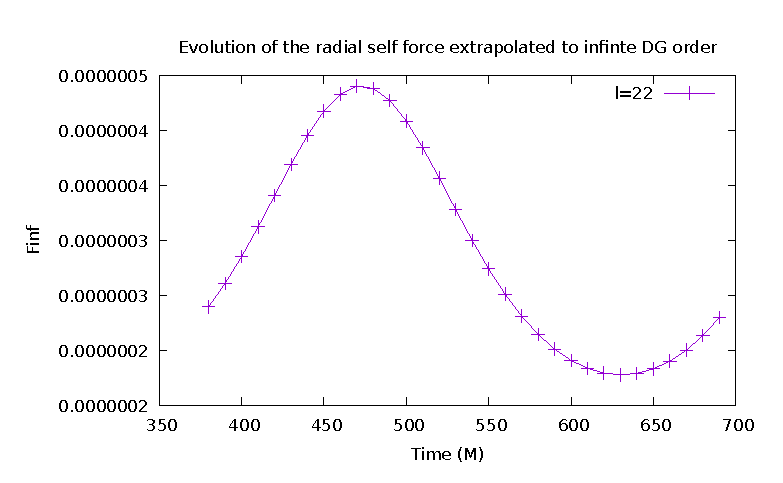
\includegraphics{/home/sdorsher/LabNotebook/20170727/finfovertimel22}
\end{figure}

\begin{figure}
  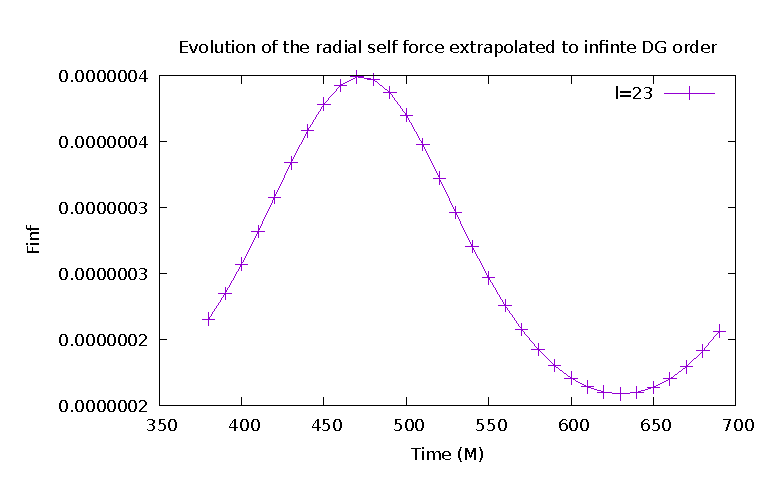
\includegraphics{/home/sdorsher/LabNotebook/20170727/finfovertimel23}
\end{figure}

\begin{figure}
  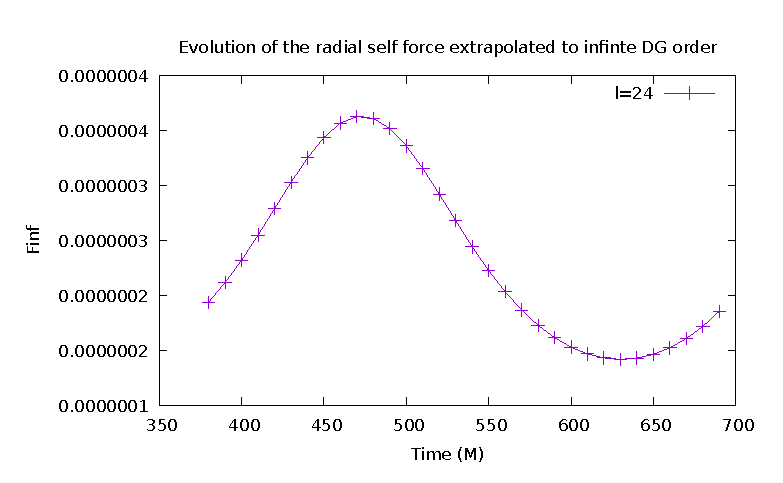
\includegraphics{/home/sdorsher/LabNotebook/20170727/finfovertimel24}
\end{figure}

\begin{figure}
  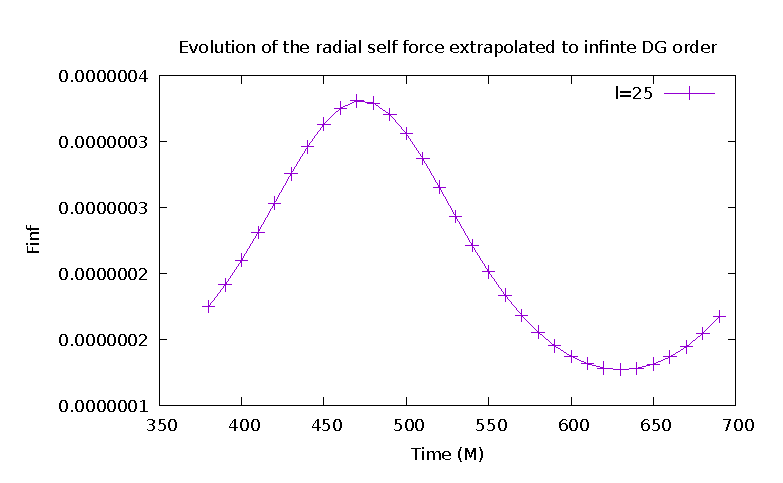
\includegraphics{/home/sdorsher/LabNotebook/20170727/finfovertimel25}
\end{figure}

\begin{figure}
  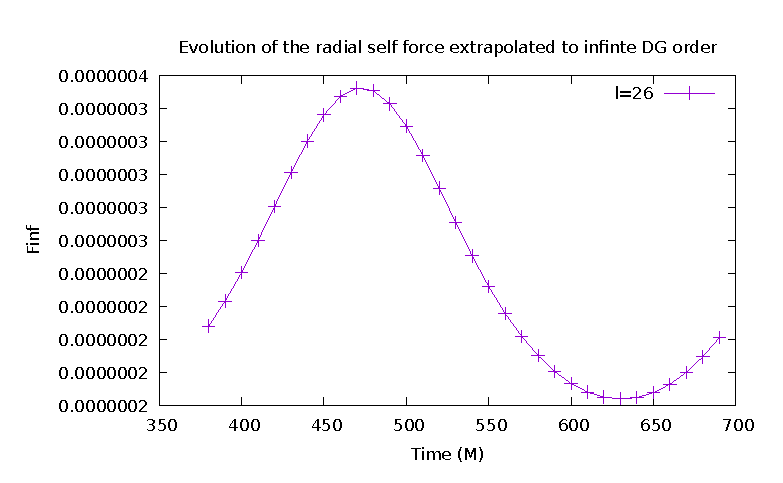
\includegraphics{/home/sdorsher/LabNotebook/20170727/finfovertimel26}
\end{figure}

\begin{figure}
  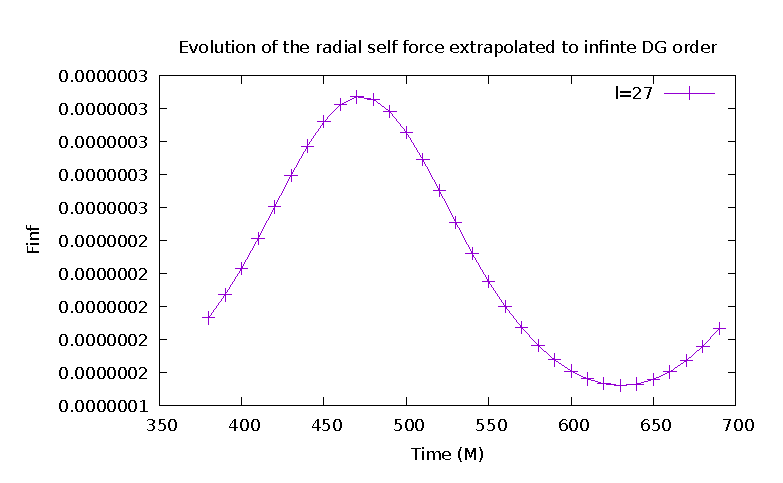
\includegraphics{/home/sdorsher/LabNotebook/20170727/finfovertimel27}
\end{figure}

\begin{figure}
  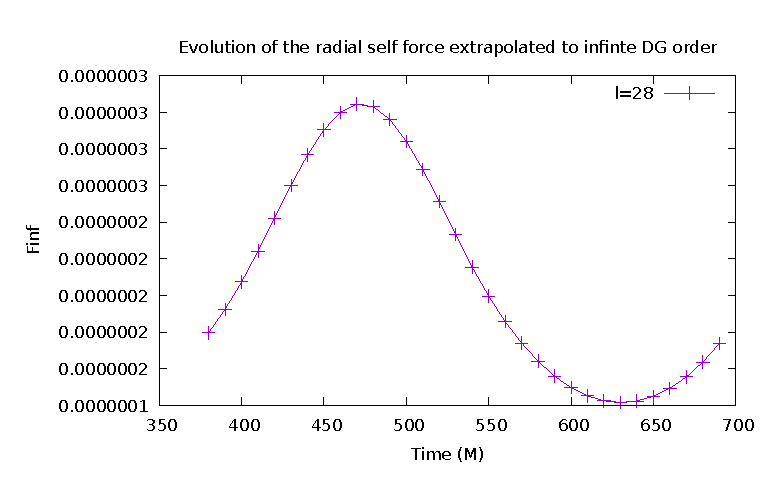
\includegraphics{/home/sdorsher/LabNotebook/20170727/finfovertimel28}
\end{figure}

\begin{figure}
  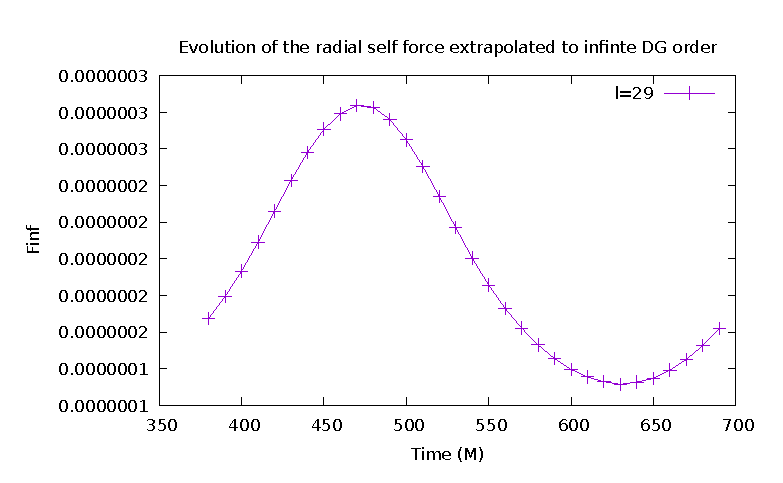
\includegraphics{/home/sdorsher/LabNotebook/20170727/finfovertimel29}
\end{figure}

\begin{figure}
  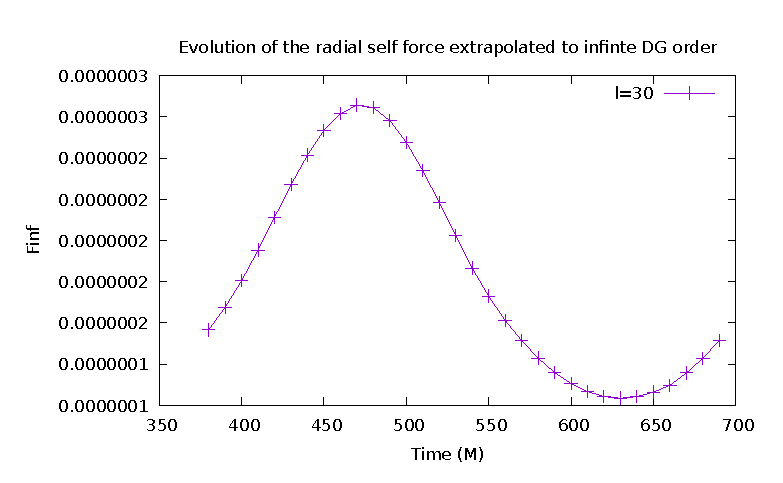
\includegraphics{/home/sdorsher/LabNotebook/20170727/finfovertimel30}
\end{figure}

\subsection{2. Sum for individual values of lmin and lmax.}

\subsection{3. Average and standard deviation of sum for individual values of lmin and lmax as a function of time}


\section{Old stuff in no particular order}






\begin{figure}
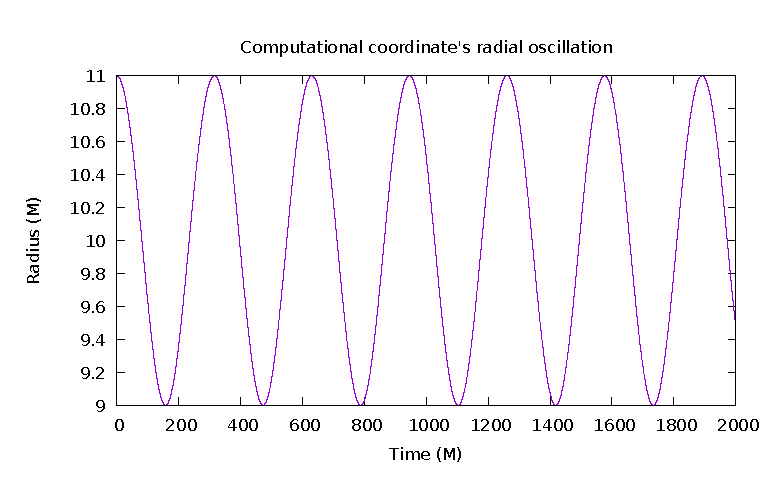
\includegraphics{/home/sdorsher/LabNotebook/20170713/orbit}
\end{figure}


\begin{figure}
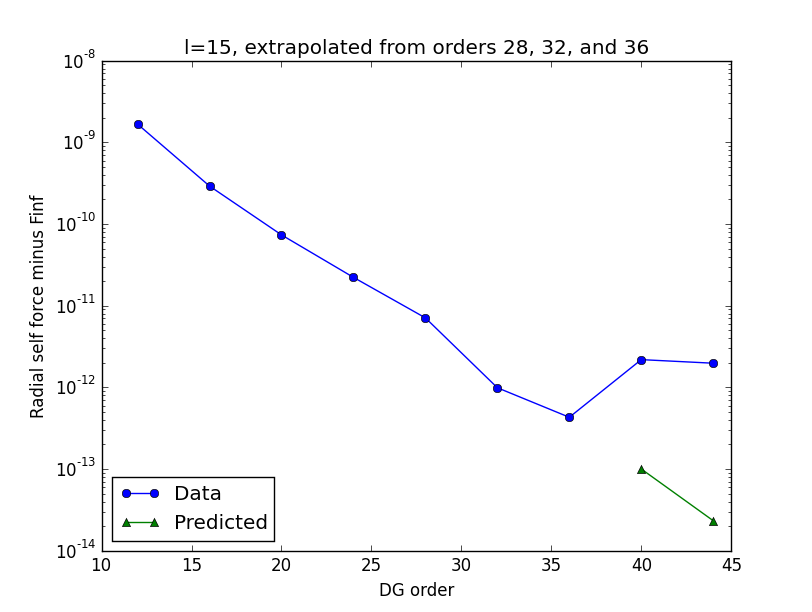
\includegraphics{/home/sdorsher/LabNotebook/20170713/extrapolate7plot}
\end{figure}

\begin{figure}
  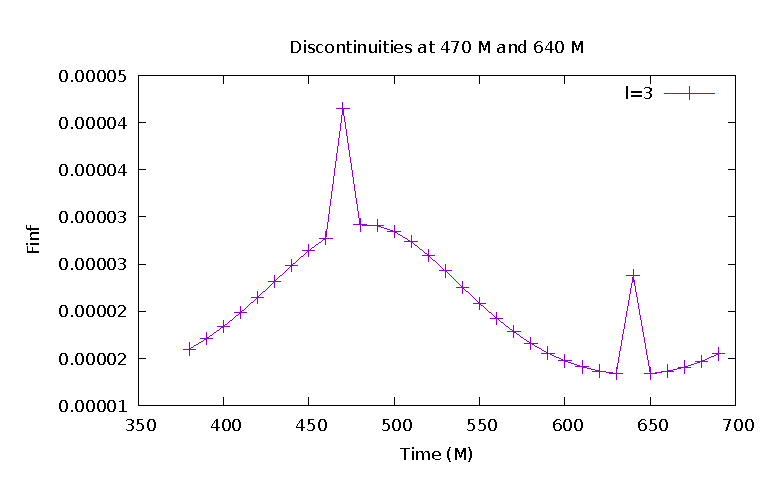
\includegraphics{/home/sdorsher/LabNotebook/20170714/finfovertimel3discontinuities}
\end{figure}


\begin{figure}
  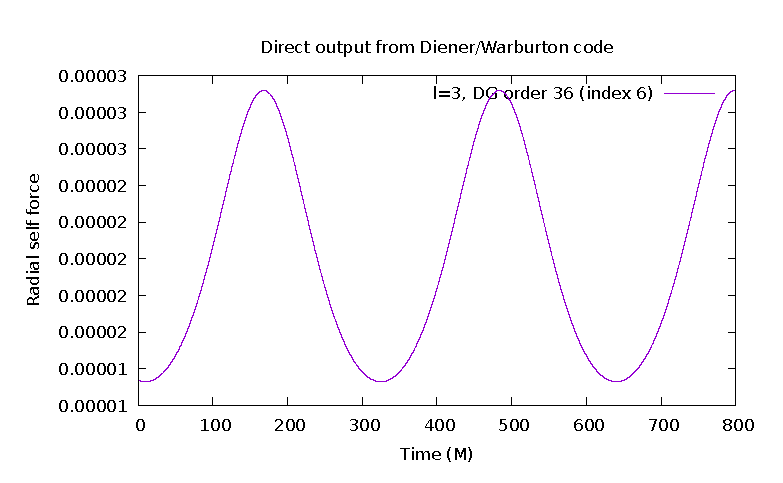
\includegraphics{/home/sdorsher/LabNotebook/20170714/psirl_l3_order36}
  \caption{470 M near perihelion, 640 M at aphelion}
\end{figure}



\begin{table}
\begin{tabular}{ll}
Starting index & finf\\
2 & 4.18128309016e-05\\
3 & mode failed\\
4 & 4.18128307505e-05\\
5 & 4.18128308245e-05\\
6 & 4.1812830828e-05\\
\end{tabular}
\end{table}


\begin{figure}
  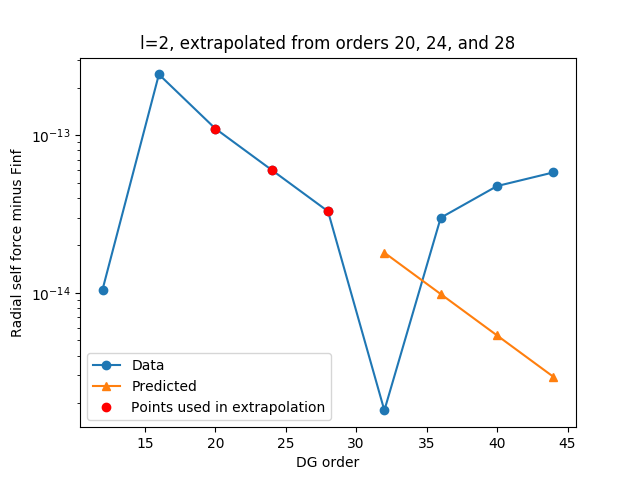
\includegraphics{/home/sdorsher/LabNotebook/20170719/extrapolate7t472l3i2}
\end{figure}

\begin{figure}
  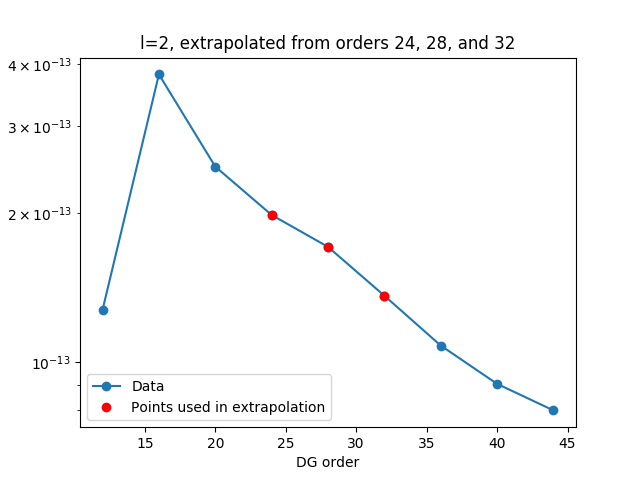
\includegraphics{/home/sdorsher/LabNotebook/20170719/extrapolate7t472l2i3}
  \caption{Note that the three points used in the extrapolation are not on a line on a semilog scale-- it is not possible to fit an exponential through them. That is why this mode failed.}
\end{figure}

\begin{figure}
  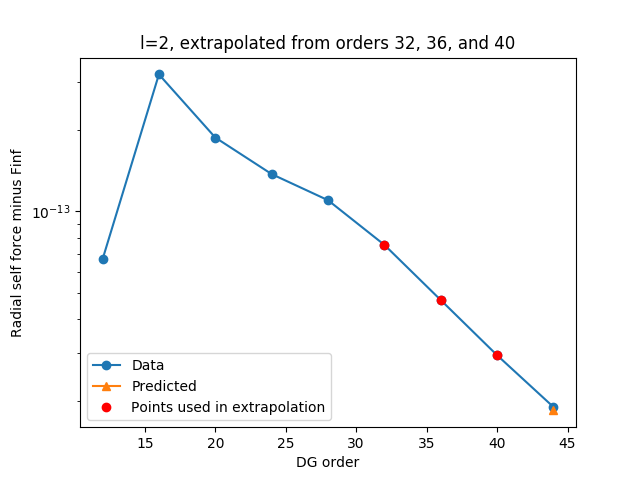
\includegraphics{/home/sdorsher/LabNotebook/20170719/extrapolate7lt472l2i5}
\end{figure}

\begin{figure}
  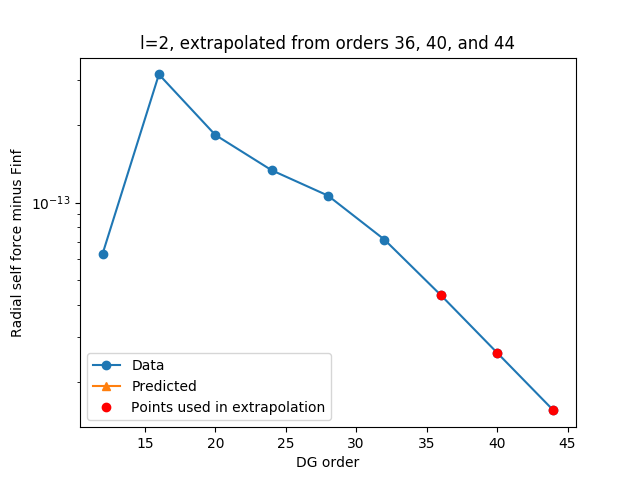
\includegraphics{/home/sdorsher/LabNotebook/20170719/extrapolate7t472l2i6}
\end{figure}

\begin{figure}
  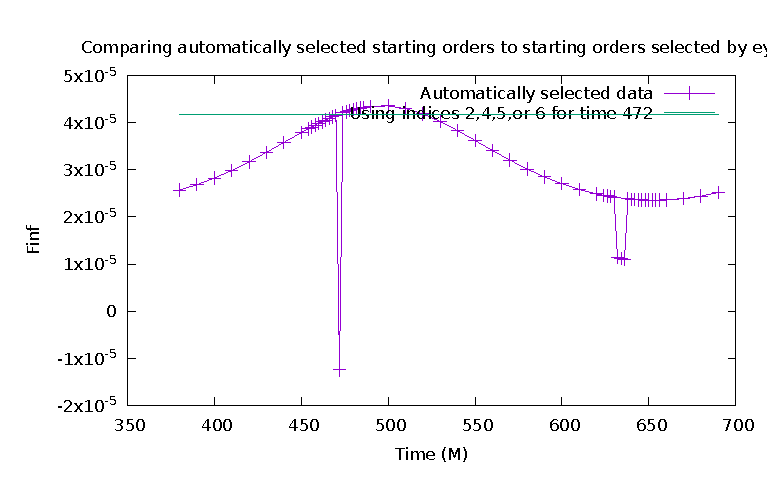
\includegraphics{/home/sdorsher/LabNotebook/20170719/manuallyChosenBestFinft472}
\end{figure}









\section{l=2}
\begin{table}
  \begin{tabular}{lll}
    time & starting order & finf\\
    632 & 0 & mode failed\\
    632 & 1 & 2.40975299617e-05\\
    632 & 2 & 2.40975300465e-05\\
    632 & 3 & 2.40975300114e-05\\
    632 & 4 & mode failed\\
    632 & 5 & 2.40975299291e-05\\
    632 & 6 & 2.40975299148e-05\\
    \hline
    634 & 0 & mode failed (however, 6 selected)\\
    634 & 1 & 2.39990698129e-05\\
    634 & 2 & 2.39990699318e-05\\
    634 & 3 & 2.39990698774e-05\\
    634 & 4 & mode failed\\
    634 & 5 & 2.39990697065e-05\\
    634 & 6 & 2.39990696758e-05\\
    \hline
    636 & 0 & mode failed (however, 6 selected)\\
    636 & 1 & 2.391047416e-05\\
    636 & 2 & 2.39104742806e-05\\
    636 & 3 & 2.39104742249e-05\\
    636 & 4 & 2.39104737911e-05\\
    636 & 5 & 2.39104739924e-05\\
    636 & 6 & 2.39104739079e-05\\
  \end{tabular}
\end{table}

\begin{figure}
  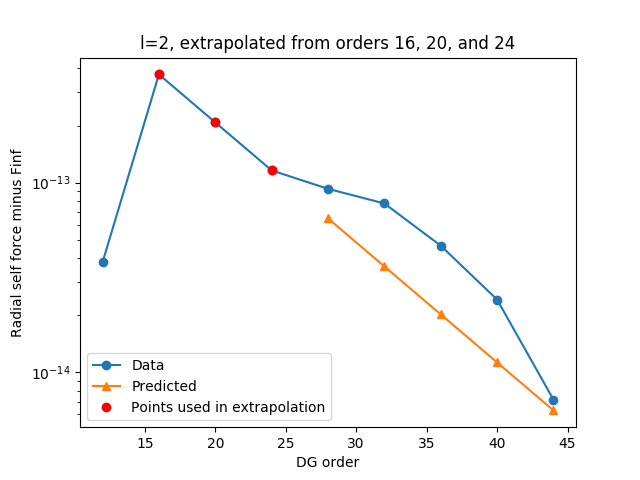
\includegraphics{/home/sdorsher/LabNotebook/20170720/extrapolate7t632l2i1}
\end{figure}

\begin{figure}
  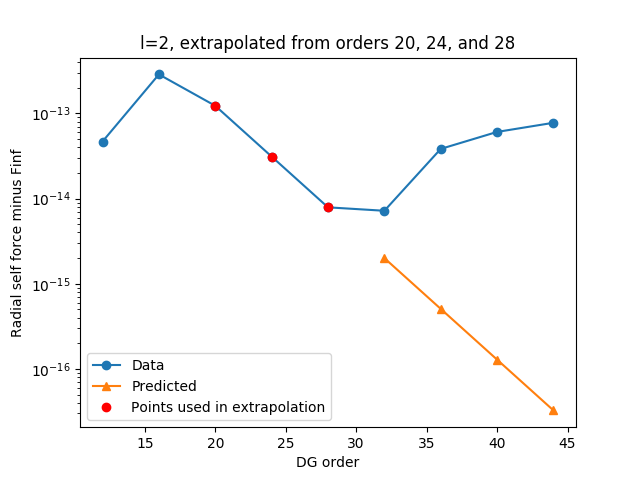
\includegraphics{/home/sdorsher/LabNotebook/20170720/extrapolate7t632l2i2}
\end{figure}

\begin{figure}
  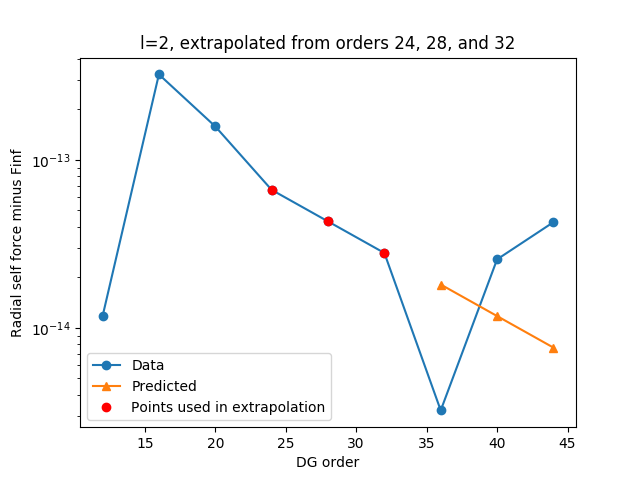
\includegraphics{/home/sdorsher/LabNotebook/20170720/extrapolate7t632l2i3}
\end{figure}

\begin{figure}
  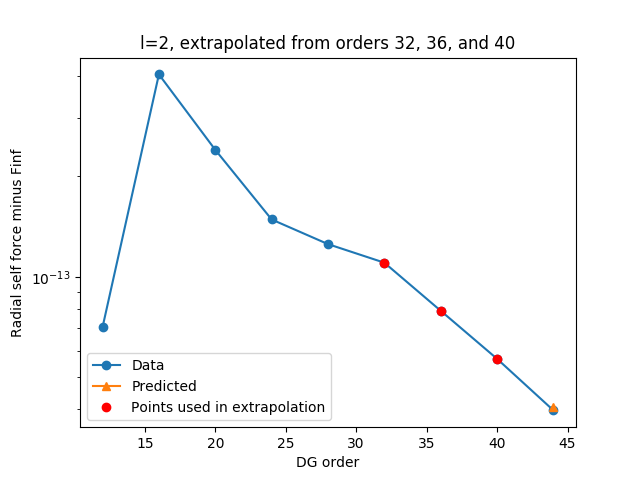
\includegraphics{/home/sdorsher/LabNotebook/20170720/extrapolate7t632l2i5}
\end{figure}

\begin{figure}
  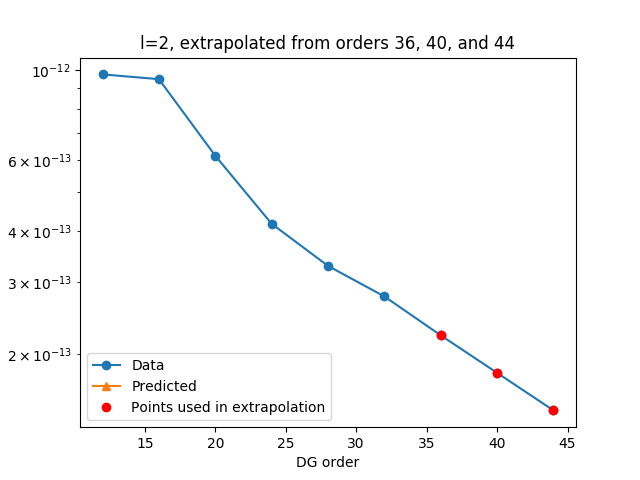
\includegraphics{/home/sdorsher/LabNotebook/20170720/extrapolate7t634l2i6}
\end{figure}

\begin{figure}
  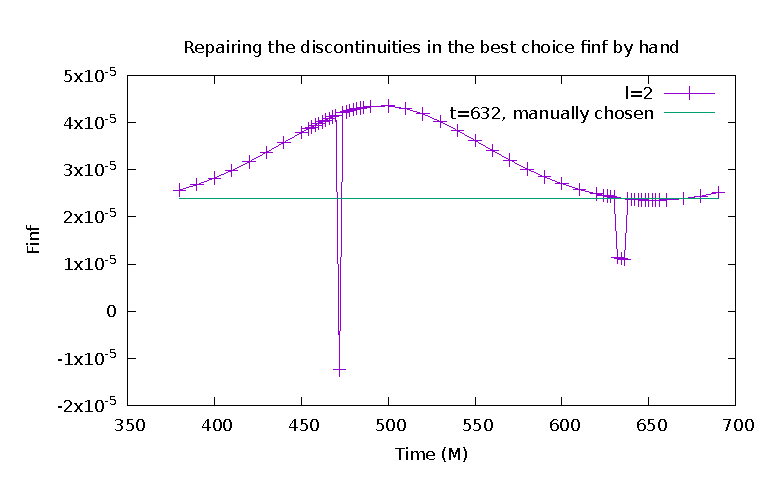
\includegraphics{/home/sdorsher/LabNotebook/20170720/bestFinfManuallyChosent632l2}
\end{figure}




\begin{figure}
  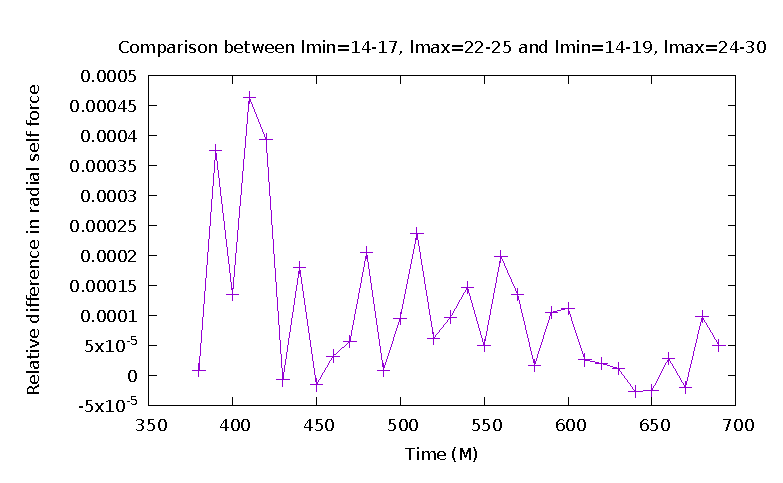
\includegraphics{/home/sdorsher/LabNotebook/20170725/relErrBigSmallRangeOverTime.eps}
  \caption{This is the relative difference between the total radial self force measured in two different ways. In both cases, the self force was extrapolated to infinite order at every l-mode at every possible DG starting order. The infinite DG order self forces over the various starting orders were sorted, eliminating NaNs. The median was chosen for each l-mode. Then the self force as a function of l-mode was fit to its three term form, and the sum was summed from zero to lmax, then extrapolated from $lmax +1 $ to infinity using an analytic form determined using Mathematica. All possible choices with lmin between 14 and 17 and lmax between 22 and 25 were averaged to obtain the total radial self force as a function of time. Similarly, all possible choices with lmin between 14 and 19 and lmax between 24 and 30 were averaged to obtain the total radial self force as a function of time. This plot shows the relative difference. I believe the smaller range is in the denominator.}
\end{figure}

\newpage

\begin{figure}
  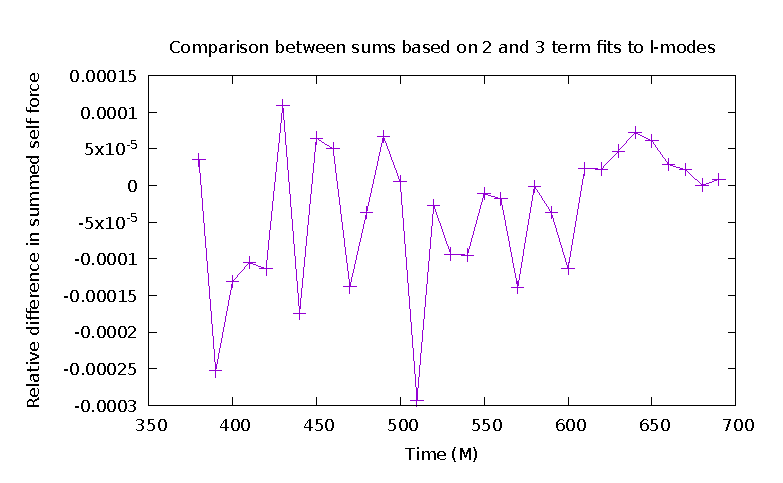
\includegraphics{/home/sdorsher/LabNotebook/20170724/relativeError23termSelfForce.eps}
  \caption{This figure was produced in the same manner as the previous figure, averaging over the smaller range, only it is a comparison between including either two or three terms in the l-mode fit. I believe the three term fit is in the denominator of the relative difference.}
\end{figure}

\begin{figure}
  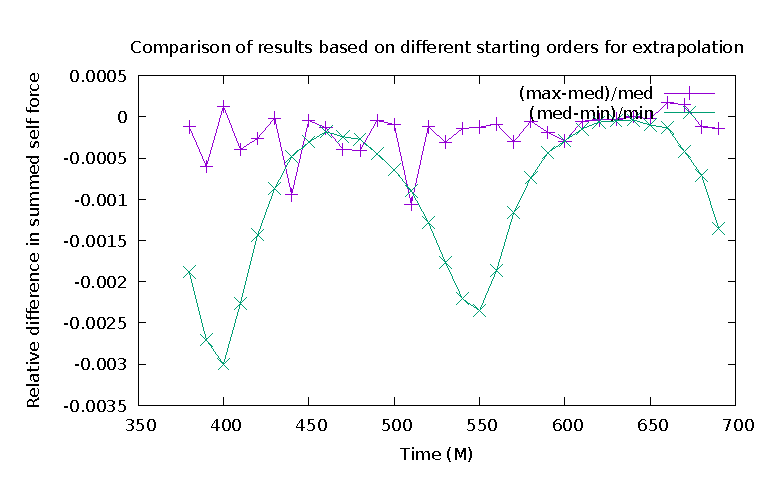
\includegraphics{/home/sdorsher/LabNotebook/20170724/minmaxmedrelativeerror3termavgl.eps}
  \caption{This figure was produced in a similar manner to the first figure, only instead of using the median, it is a comparison between using the median, the maximum, and the minimum. The purple line is the relative difference between the maximum and the median, which is subject to roundoff error due to the potential for the maximum to contian roundoff error. The green line is the relative difference between the median and the minimum, which is subject to effects due to failure to converge. I suspect the median is the best compromise between these two effects, rejecting outliers in both directions, though it is a simplistic approach to doing so, and does not guarantee success. It is possible to have a starting order that has not converged and is also in the roundoff regime, for example. A better guarantee of success, though not a certain one, would be to do a fit over part of the error convergence plot to determine exponentiality, by fitting a line in semilog scale. However, this seems unnecessarily complex at this time.}
\end{figure}
  
\begin{figure}
  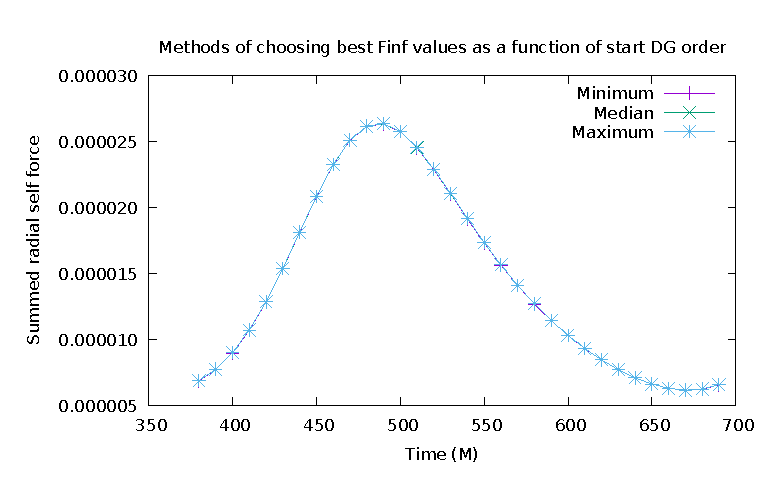
\includegraphics{/home/sdorsher/LabNotebook/20170724/bestfinfscriptplot.eps}
  \caption{This is the actual summed, doubly extrapolated, radial self force, measured in three different ways as described in the three figures above.}
\end{figure}






\end{document}
